In general, we did execute our plan (given in the previous submission) for the actual implementation, with only slight changes outlined below (Section \ref{sec_differences}). In the final implementation of the metal manufacturing simulation we implemented two cooperation mechanisms; the prospector agents employ implicit cooperation for the assignment of sub-areas of the map, and the digger agents and the digger coordinator cooperate via coalitions and contract net to distribute the mining tasks. 

\subsection{Prospectors: Implicit Coordination}

Initially, the list of sub-areas to observe is empty. The Prospector Coordinator (PC) then separates the map into as many sub-areas as there are prospectors in the system. This division is approximate, the algorithm tries to make this sub-areas as equally-sized as possible, but in order to ensure that the areas are compact, they may be slightly different. The algorithm ensures that all cells are assigned to one group, but it does not guarantee that all groups are equally sized. Figure \ref{fig:map_division} shows some examples of this division using different number of prospectors.

\begin{figure}[H]
	\centering
	\subfigure[Division with 2 prospectors]{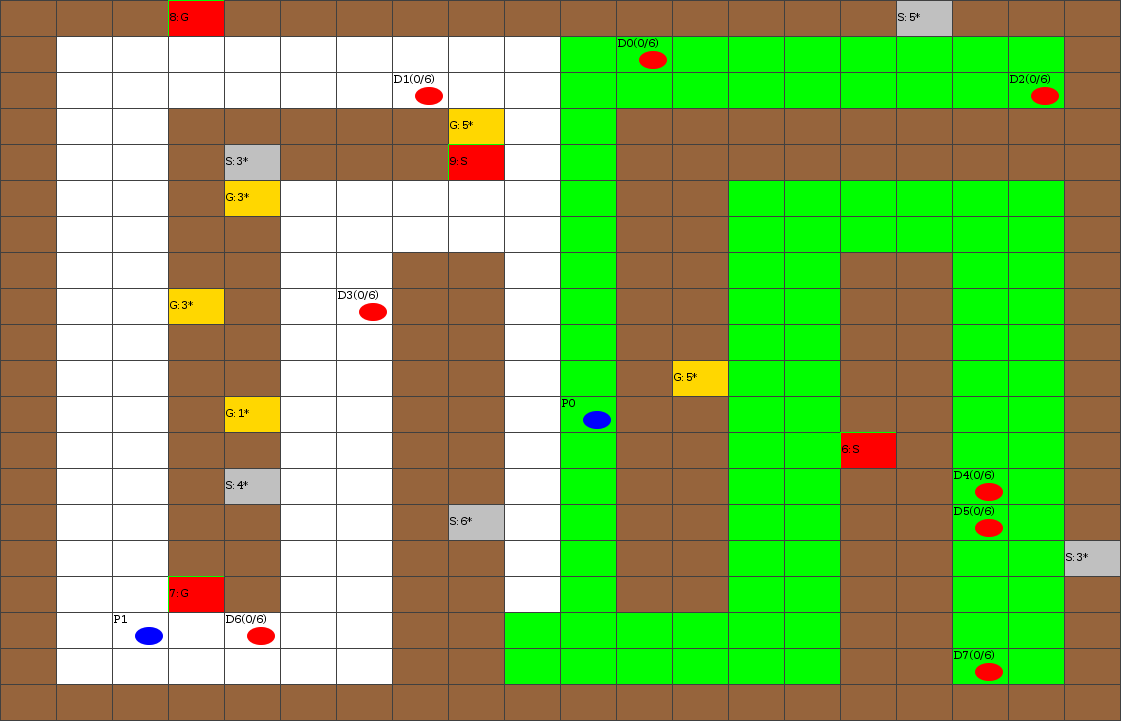
\includegraphics[width=0.49\textwidth]{images/2prospectors_image.png}}
	\subfigure[Division with 4 prospectors]{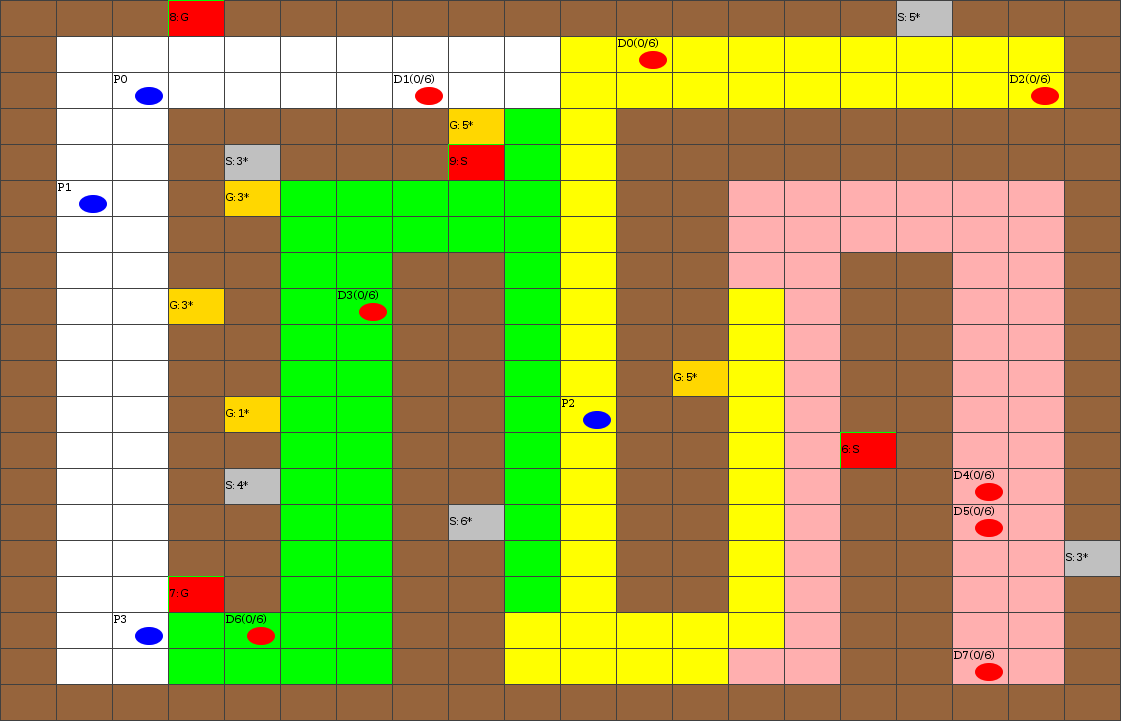
\includegraphics[width=0.49\textwidth]{images/4prospectors_image.png}}
	\subfigure[Division with 7 prospectors]{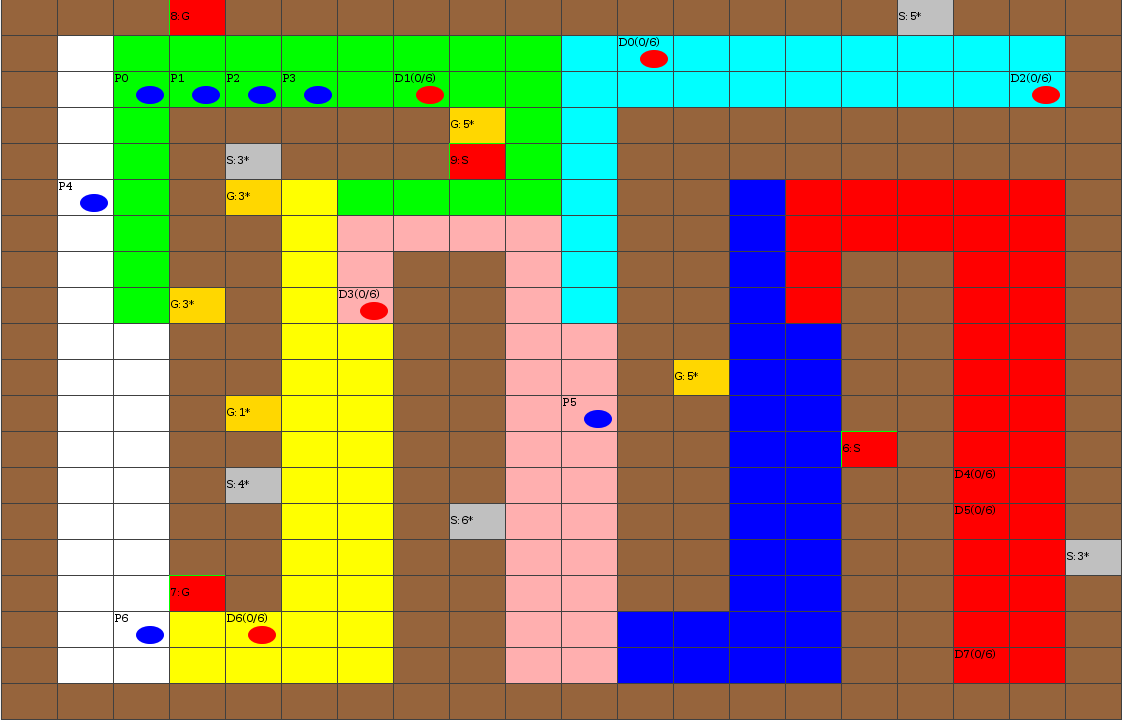
\includegraphics[width=0.49\textwidth]{images/7prospectors_image.png}}
	\subfigure[Division with 8 prospectors]{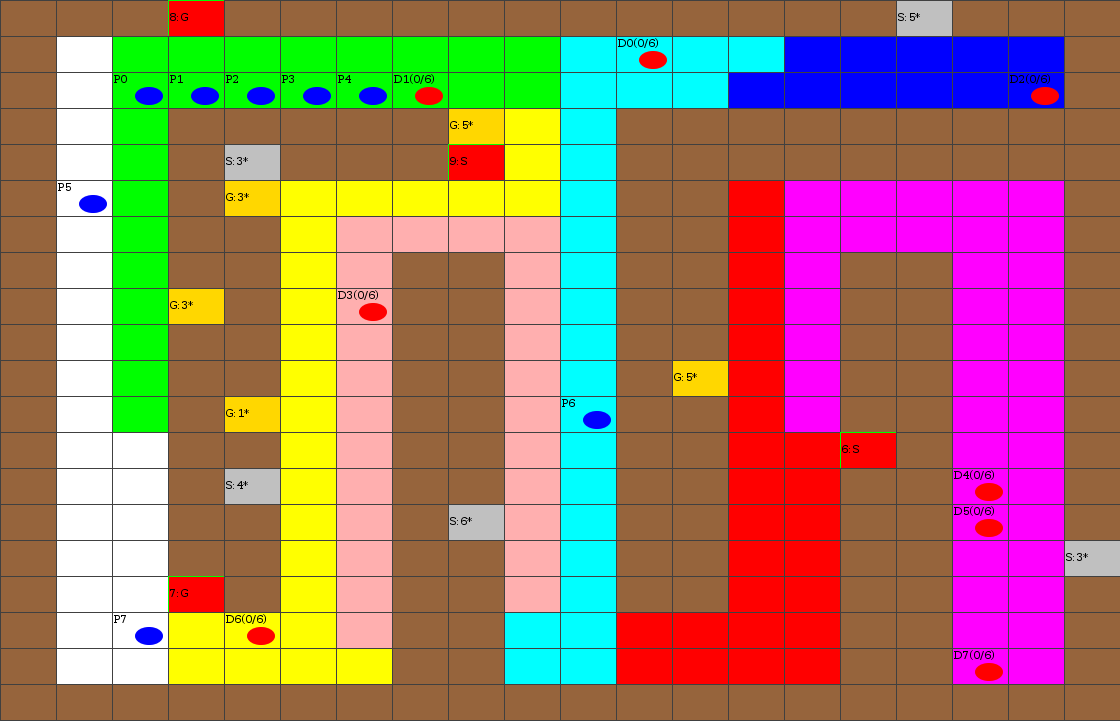
\includegraphics[width=0.49\textwidth]{images/8prospectors_image.png}}
	\caption{Map distribution for different number of prospectors.}
	\label{fig:map_division}
\end{figure}


Those sub-areas are added to a synchronous list within the gameSettings object sent to all prospectors at each round. Then each prospector will decide which are the most convenient areas and it will create an ordered list of preference that will be sent to the Prospector coordinator. 

Finally the prospector coordinator, will get the preference lists from the prospectors and it will assign the preferred area for each prospector from the remaining ones. Therefore, the first prospector to send the message will surely get its preferred option, but once assigned, the sub-area will be removed from the list of available sub-ares. Consequently, any agent with the same preferred option will be assigned with a less preferred option.

Once all the agents have a sub-area of the map assigned, they will go there and start exploring. Prospectors do the exploration by selecting the next move based on the number of times a cell has been explored before, remembering the places where it has been before. So at each round, each prospector will move to the least explored cell from the accessible ones. 

In the worst case scenario multiple agents select the same sub-area to observe as the preferred one. This problem could be solved implementing a more sophisticated mechanism like, for example, Contract Net. However, an unfair distribution of the sub-areas only has an impact in the first rounds of the simulation when the prospectors need to move to their assigned area; it will later be irrelevant as they will already be in their assigned areas. 

This solution was relatively simple to implement, and did not need require any complex calculations for finding the best distribution, or communication between the agents.


\subsection{Diggers: Contract Net}

To distribute the mining tasks amongst the digger agents we implemented Contract Net.

Digger Coordinator Agent - DelegateTasksBehaviour:
During the first stage, the Digger Coordinator agent assesses the current state and recognizes if there is metal which still need to be assigned to a digger agent. The Digger Coordinator then adds the task to the list which will include its constraints, like which metal and how many units are involved, and where is it located. 

Digger Coordinator Agent -TaskContractNetInitiatorBehaviour:
Announcements of new tasks are broadcasted to all of the digger agents. After all of the digger agents reply, the Digger coordinator accepts the best proposal. 

Digger Agents - TaskContractNetResponderBehaviour:
Each Agent decides if they want to bid for the task, depending on the type of metal and its carrying capacity, and sends a proposal or refuses.

We don’t consider the manufacturing of the ore to be part of the coordination mechanisms. This is handled implicitly by each agent, based on the amount of ore they are carrying, the distance from the manufacturing centers and the price each manufacturing center pays for one unit of the metal.


Additionally we changed the strategy for giving out the tasks for the digger agents. The tasks are sorted by the distance/points ratio (distance to the next manufacturing center plus rounds to finish collection and total points paid for the amount of metal the agent is carrying) before they are announced sequentially for the contract net. This leads to diggers working in the neighborhood of the manufacturing centers as long as there is ore available, and speeds up the collection process. As shown in table 1, the average time for collecting the metal when sorting the tasks is less than the half of the time without sorting, and we obtain an increase of more than 50\% in the total benefits.

\begin{table}[H]
	\begin{center}
		\scalebox{0.9}{
			\begin{tabular}{c|c|c}
			& \textbf{without sorting} & \textbf{sorted pointsPerRound} \\\hline
			Total benefits & 3784 & 5773 \\
			Total SILVER manufactured & 238 & 381 \\
			Total GOLD manufactured & 233 & 332 \\
			Total metal manufactured & 471 & 713 \\
			Average benefit per unit & 8.03 & 8.1 \\
			Average time for discovery & 35.33 & 35.86 \\
			Average time for collection & 202.26 & 87.42 \\
			Total metal on map & 1208 & 1476 \\
			Ratio of discovered metal & 0.97 & 0.94 \\
			Ratio of collected metal & 0.39 & 0.48 \\
			\end{tabular}

		}
	\end{center}
	\caption{Statistics after round 600.}
	\label{tab:summary}
\end{table}